% !TeX spellcheck = en_GB
\documentclass[usenames,dvipsnames,aspectratio=169]{beamer}
\usepackage{tcolorbox} % Add this package
\usepackage{tikz}
\usetikzlibrary{shadows, positioning, shapes.geometric, arrows.meta, fit, decorations.pathmorphing, er}
\usepackage{pgfplots}
\usepackage{pgfplotstable}
\usepackage{pgf-pie}
\usepackage{graphicx}
\usetheme{Szeged}
\usecolortheme{beaver}


% Define custom colors for Elixir
\definecolor{ElixirPurple}{RGB}{104, 55, 155} % Adjust the RGB values to match Elixir's purple
\definecolor{ElixirLightPurple}{RGB}{170, 120, 210} % A lighter shade of purple
\definecolor{ElixirVeryLightPurple}{RGB}{230, 220, 250} % A very light shade of purple for the background


% Setting color of bars
% Setting colors for the bars and title
\setbeamercolor{palette primary}{bg=ElixirPurple,fg=white}
\setbeamercolor{palette secondary}{bg=ElixirLightPurple,fg=white}
\setbeamercolor{palette tertiary}{bg=ElixirPurple,fg=white}
\setbeamercolor{palette quaternary}{bg=ElixirPurple,fg=white}
\setbeamercolor{titlelike}{parent=palette primary, fg=white}
\setbeamercolor{frametitle}{fg=white,bg=ElixirPurple}
\setbeamercolor{background canvas}{bg=ElixirVeryLightPurple}


% Set item colors
\setbeamercolor{item}{fg=ElixirPurple}
\setbeamercolor{itemize item}{fg=ElixirPurple}
\setbeamercolor{itemize subitem}{fg=ElixirPurple}


\title{Sentiment Analysis on Mastodon Posts}
\subtitle{Predicting Election Outcomes with Elixir?}
\author{Sebastian Heiden}
\institute{Harz University of Applied Sciences}
\date{\today}

\newcommand{\graybar}[4]{
	\begin{tikzpicture}[remember picture, overlay]
		\node at (current page.north west) [anchor=north west, xshift=#1, yshift=#2] {
			\begin{tikzpicture}
				\draw[fill=gray!10, draw=none] (0, 0) rectangle (#3, -#4);
			\end{tikzpicture}
		};
	\end{tikzpicture}
}



% Define a custom command for post-it notes
% Arguments:
% 1: Horizontal shift (positive value moves right, negative left)
% 2: Vertical shift (positive value moves up, negative down)
% 3: Width of the post-it note
% 4: Text to be placed in the post-it note
\newcommand{\postitnote}[4]{
	\begin{tikzpicture}[remember picture, overlay]
		\node[anchor=north west, 
		xshift=#1, 
		yshift=#2, 
		fill=yellow!40, 
		draw=black, 
		thick, 
		text width=#3, 
		rounded corners, 
		drop shadow] 
		at (current page.north west) 
		{#4};
	\end{tikzpicture}
}


\logo{
\includegraphics[height=1cm]{pictures/LogoElixirBerlin.png}} % Adjust size as needed

\begin{document}
	
	{
		\setbeamertemplate{headline}{} % Removes header from title page
		\begin{frame}
			\titlepage
		\end{frame}
	}
	
	% Your other slides go here
	
	\section{About Me}
	% !TeX spellcheck = en_GB

\pgfplotsset{compat=1.17}

\begin{frame}{About Me}
	\begin{columns}
		
		\begin{column}{0.45\textwidth}
			\begin{tcolorbox}[colback=white, colframe=ElixirPurple, arc=3mm, boxrule=0mm, height=0.8\textheight, valign=center, title=Working Live]
				
				\underline{topics}:
				\begin{itemize}
					\item heat demand and PV cadastres
				\end{itemize}
				\underline{using}:
				\begin{itemize}
					\item geodata (Raster, Vector)
					\item Python: GeoPandas, Numpy
					\item land usage; coverage, property register
				\end{itemize}
				
			\end{tcolorbox}
		\end{column}
		
		\begin{column}{0.45\textwidth}
			\begin{tcolorbox}[colback=white, colframe=ElixirPurple, arc=3mm, boxrule=0mm, height=0.8\textheight, valign=center, title=Privat Live]
				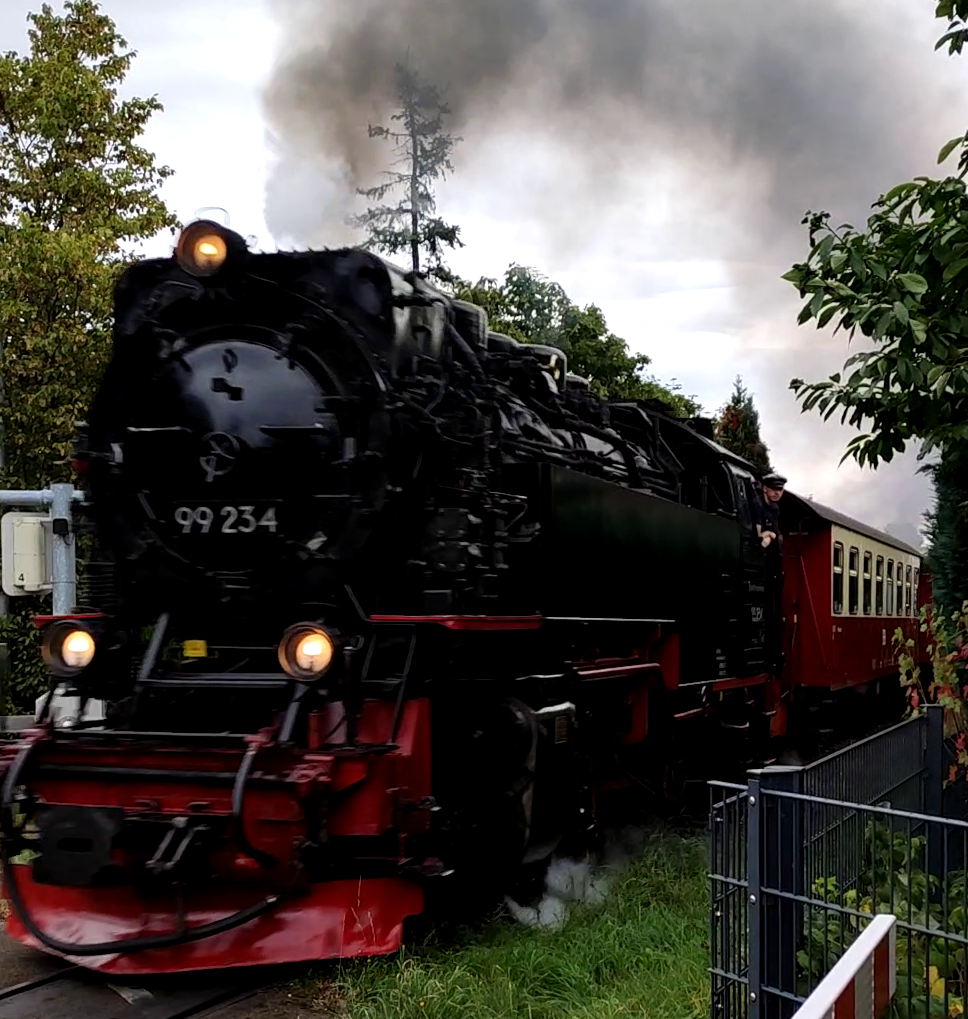
\includegraphics[width=\tcbtextwidth,   keepaspectratio]{pictures/vlcsnap-2024-01-31-23h37m06s479.png}
			\end{tcolorbox}
		\end{column}
		
	\end{columns}
\end{frame}
	
	\section{Motivation}
	% !TeX spellcheck = en_GB

\begin{frame}{Election Monitoring with on Twitter~\footfullcite{attarwala_how_2017}}
	\vspace*{-1.2mm}
	\begin{figure}
		\centering
		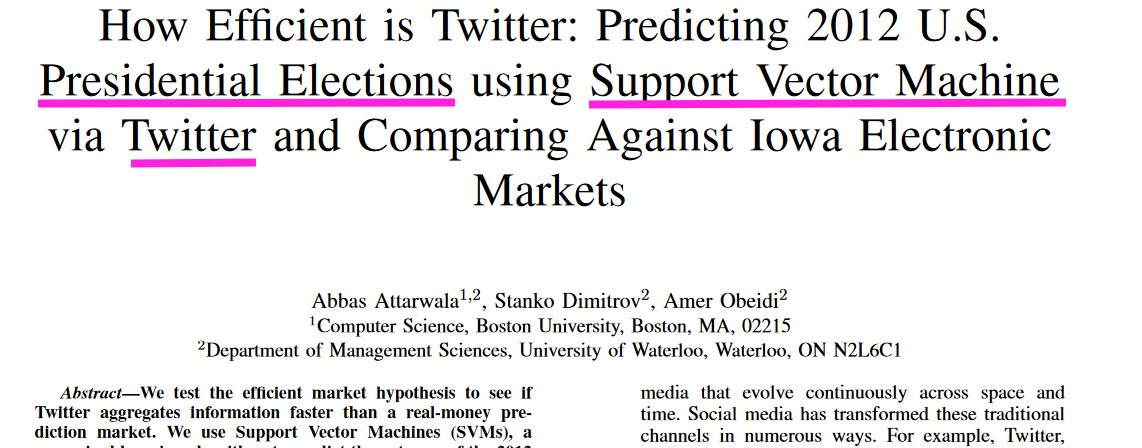
\includegraphics[width=0.9\linewidth, keepaspectratio]{pictures/TwitterElection2012/Twitter_Election_2012_small.png}
	\end{figure}

\end{frame}


\begin{frame}{Prediction}
	\begin{columns}
		
		\begin{column}{0.55\textwidth}
			\begin{tcolorbox}[enhanced jigsaw, colback=white, opacityback=.4, colframe=ElixirPurple, arc=3mm, boxrule=0mm, height=0.8\textheight, valign=center, title=Frequency]
				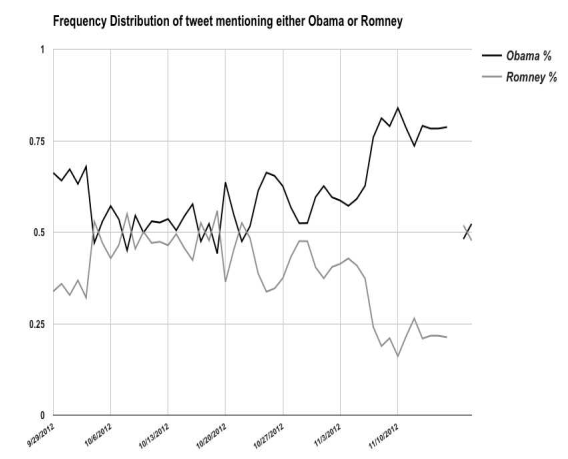
\includegraphics[width=\tcbtextwidth,   keepaspectratio]{pictures/TwitterElection2012/twitter_temp_distr.png}
			\end{tcolorbox}
		\end{column}
		
		\begin{column}{0.55\textwidth}
			\begin{tcolorbox}[enhanced jigsaw, colback=white, opacityback=.4, colframe=ElixirPurple, arc=3mm, boxrule=0mm, height=0.8\textheight, valign=center, title=Prediction]
				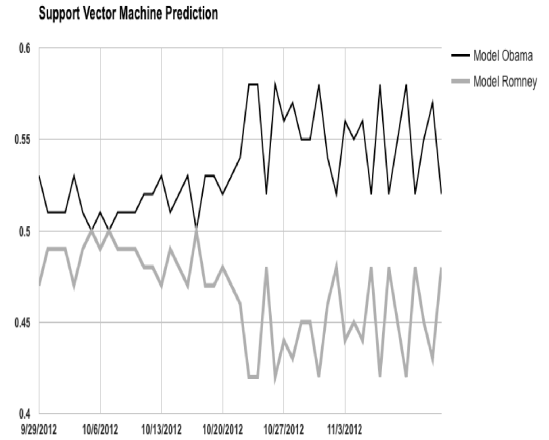
\includegraphics[width=\tcbtextwidth,   keepaspectratio]{pictures/TwitterElection2012/twitter_svm.png}
			\end{tcolorbox}
		\end{column}
		
	\end{columns}
\end{frame}


\begin{frame}{Election on Mastodon}
	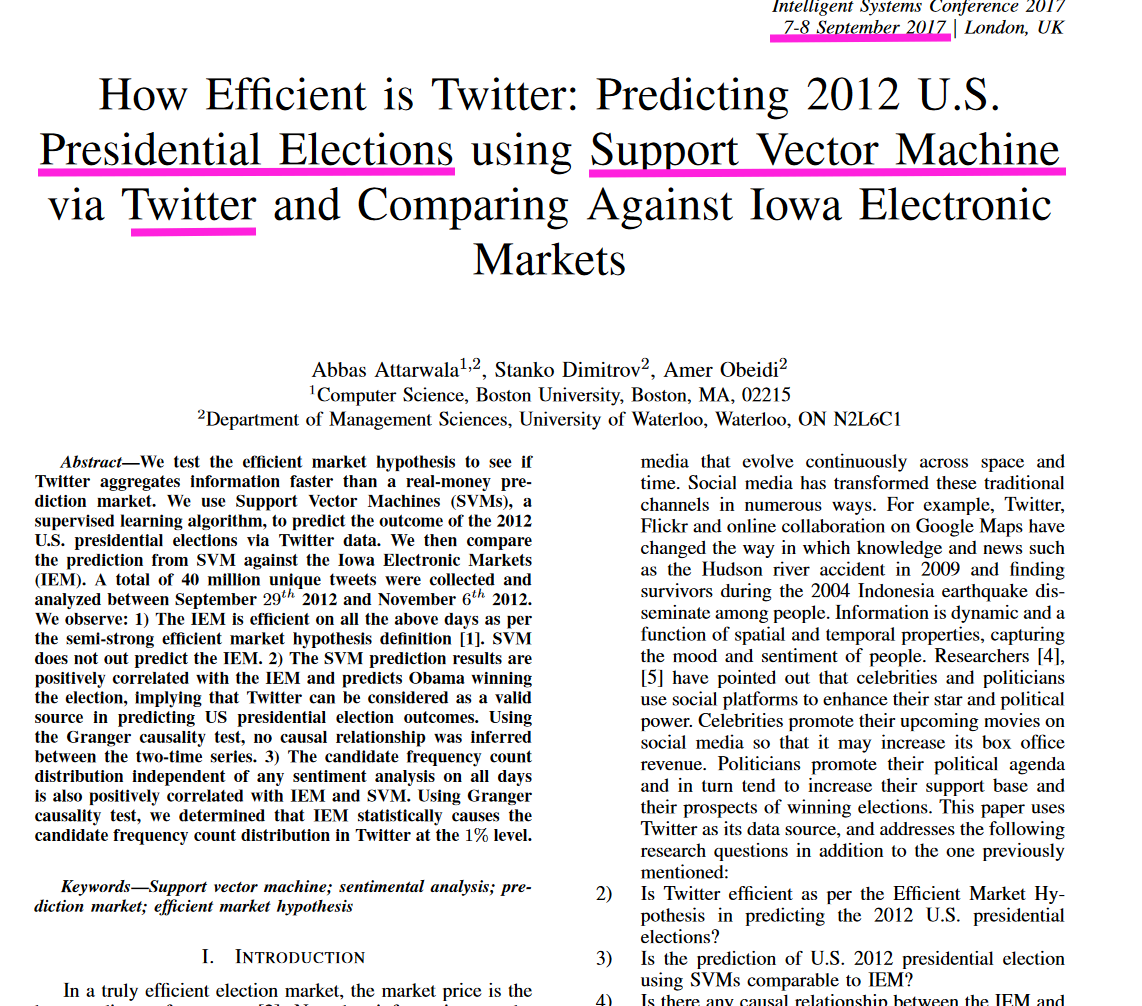
\includegraphics[width=\linewidth, keepaspectratio]{pictures/TwitterElection2012/Twitter_Election_2012.png}
	\postitnote{1.5cm}{-3.5cm}{4.8cm}{Bavarian State Election}
	\postitnote{8.2cm}{-3.5cm}{6.5cm}{Pre-Trained Deep Learning NLP Model}
	
	
	\postitnote{6.1cm}{-2.8cm}{1.8cm}{Mastodon}
	\postitnote{10.8cm}{-2.8cm}{2.5cm}{2023}
	
	\graybar{4.1cm}{-4.1cm}{10.8cm}{2.0cm}
	\postitnote{2.3cm}{-4.2cm}{1.8cm}{Mastodon}
	
\end{frame}

	
	\section{DS Background}
	% !TeX spellcheck = en_GB

\begin{frame}{Data Science \& Big Data \footnote{Courtesy Prof. F. Transchel, Harz University of Applied Sciences.}}
	\begin{columns}
		
		\begin{column}{0.75\textwidth}
			\begin{tcolorbox}[enhanced jigsaw, colback=white, opacityback=.4, colframe=ElixirPurple, arc=3mm, boxrule=0mm, height=0.75\textheight, valign=center, title=DS Perspective]
					\begin{figure}[htbp]
					\centering
					\resizebox{0.93\columnwidth}{!}{% !TeX spellcheck = en_GB

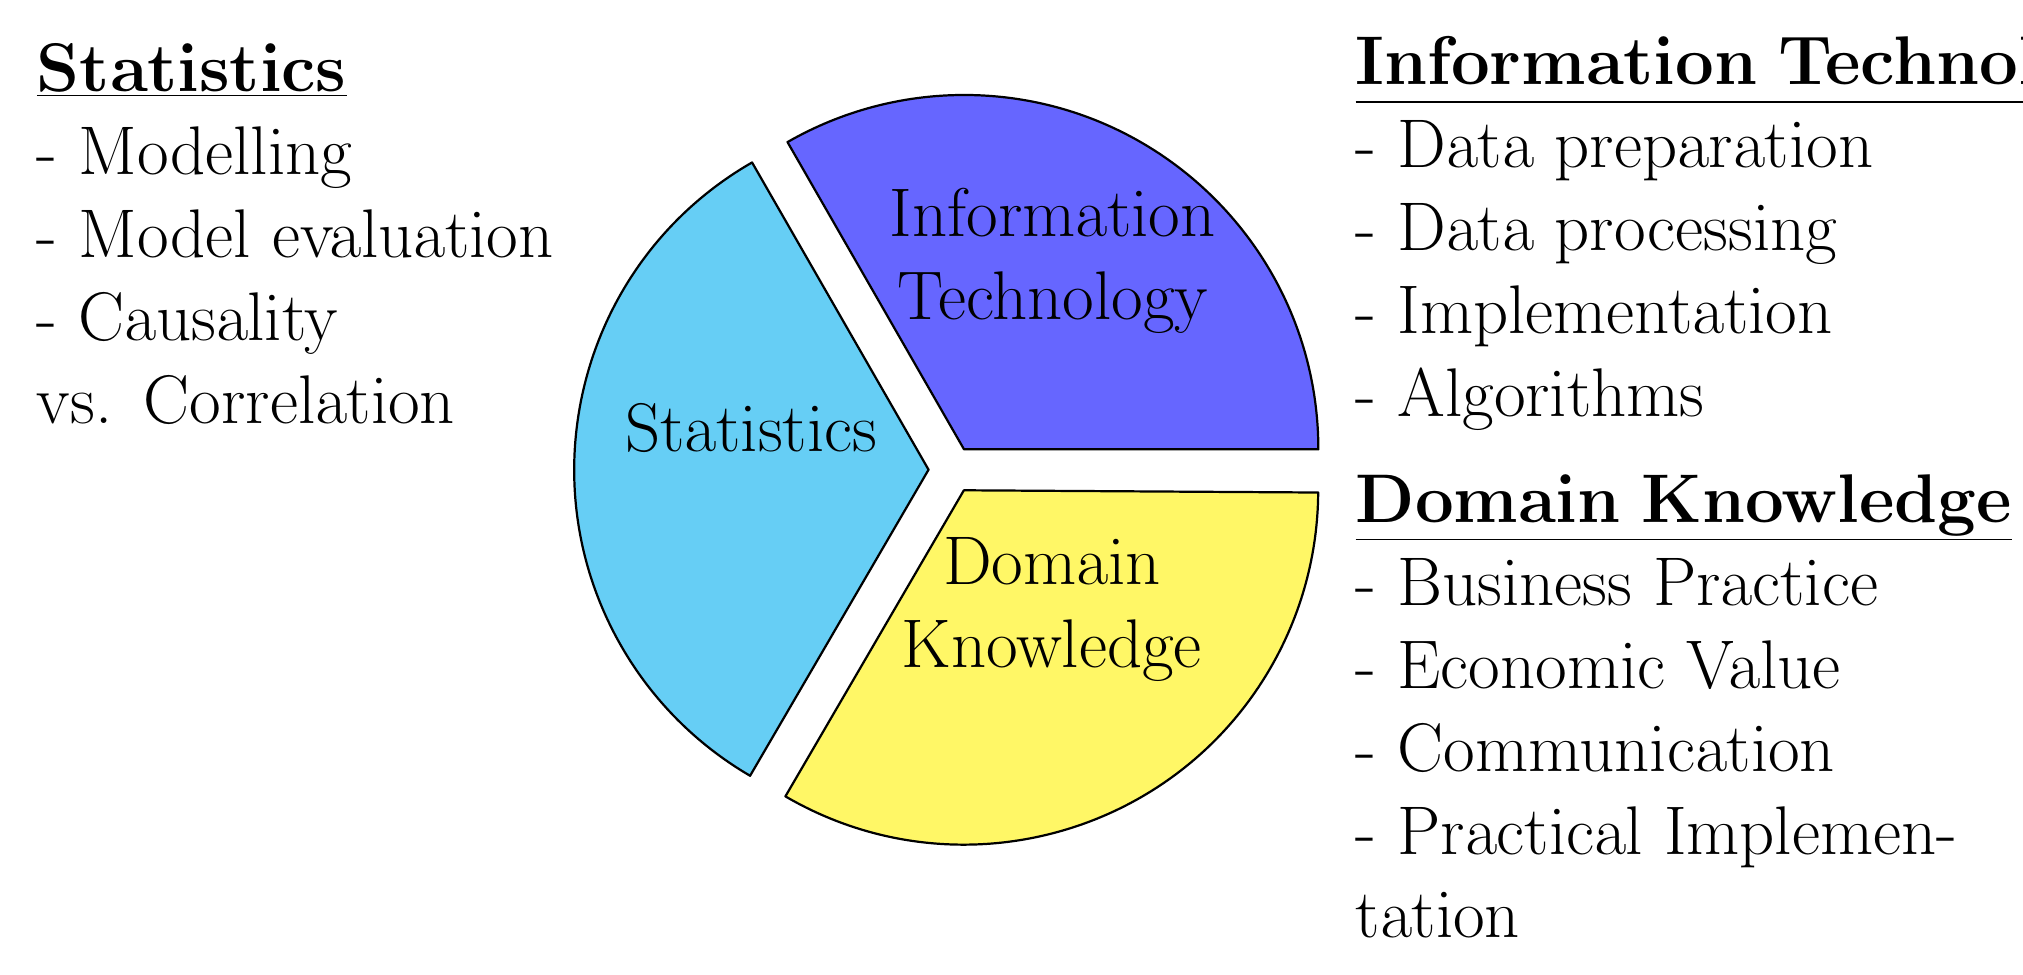
\begin{tikzpicture}[every node/.style={font=\Huge}]

	% Draw the pie chart with separated slices
	\pie[explode=0.3, text=inside, radius=4.5, hide number]{
		33.3/Information \\ Technology,
		33.3/Statistics,
		33.3/Domain \\ Knowledge
	}
	
	% Add legends or annotations
	\node[align=left, anchor=west, text width=7cm] at (5, 3) {
		\underline{\textbf{Information Technology}}\\
		- Data preparation\\
		- Data processing\\
		- Implementation\\
		- Algorithms
	};
	
	\node[align=left, anchor=east, text width=8cm] at (-3.5, 3) {
		\underline{\textbf{Statistics}}\\
		- Modelling\\
		- Model evaluation\\
		- Causality \\ vs. Correlation
	};
	
	\node[align=left, anchor=west, text width=8cm] at (5, -3) {
		\underline{\textbf{Domain Knowledge}}\\
		- Business Practice\\
		- Economic Value\\
		- Communication\\
		- Practical Implementation
	};
\end{tikzpicture}}
					\caption{High Level}
				\end{figure}
			\end{tcolorbox}
		\end{column}
		
		\begin{column}{0.25\textwidth}
			\begin{tcolorbox}[enhanced jigsaw, colback=white, opacityback=.4, colframe=ElixirPurple, arc=3mm, boxrule=0mm, height=0.75\textheight, valign=center, title=Big Data]
				
				\begin{itemize}
					\item Volume
					\item Velocity
					\item Variety
					\vspace{3pt}
					\item Veracity
					\vspace{3pt}
					\item Value
					\item Validity
					
				\end{itemize}
				
			\end{tcolorbox}
		\end{column}
	\end{columns}
\end{frame}

\begin{frame}{CRISP-DM}
	\begin{figure}[htbp]
		\centering
		\resizebox{\columnwidth}{!}{% !TeX spellcheck = en_GB

\definecolor{walnut}{RGB}{61, 43, 31}  % Deep, dark brown color akin to walnut

\tikzset{
	block/.style={
		rectangle,
		draw,
		fill=yellow!30,
		text width=7em,
		text centered,
		rounded corners=3mm,
		minimum height=4em,
		line width=0.7mm,
	},
	arrow/.style={
		thick,
		-{Latex[length=3mm,width=3mm]},
		line width=1mm,
		walnut % Adjusted color
	},
	doublearrow/.style={
		thick,
		{Latex[length=3mm,width=3mm]}-{Latex[length=3mm,width=3mm]},
		line width=1mm,
		walnut % Adjusted color
	},
	decision/.style={
		diamond,
		draw,
		fill=blue!20,
		text width=4.5em,
		text badly centered,
		node distance=3cm,
		inner sep=0pt,
		thick
	},
	dashedarrow/.style={ % Style for dashed arrow
		thick,
		-{Latex[length=3mm,width=3mm]},
		line width=1mm,
		walnut, % Adjusted color
		dashed
	}
}

\begin{tikzpicture}[node distance=1.2cm and 3.5cm]
	% Place nodes
	\node [block] (business) {Business understanding};
	\node [block, right=4.5cm of business] (dataund) {Data understanding};
	\node [block, right=3.0cm of dataund] (dataprep) {Data preparation};
	\node [block, below=of dataprep] (modeling) {Modelling};
	\node [block, below=of dataund] (evaluation) {Evaluation};
	\node [block, below=of business, align=center] (implementation) {Implementation\\into production};
	
	% Draw edges
	\draw [arrow] (dataund) -- (dataprep);
	\draw [doublearrow] (dataprep) -- (modeling); % Arrow starts from the center of the node
	\draw [arrow] (modeling) -- (evaluation);
	\draw [arrow] (evaluation) -- (implementation); % Arrow with head on both ends

	\draw [doublearrow] (business) -- (dataund); % Arrow with head on both ends
	\draw [dashedarrow] (evaluation) -- (business);
	
	% Source text, aligned with the 'Business understanding' node
	\node[anchor=north west, align=left, text width=15cm, below=of implementation, yshift=1cm, xshift=6cm] (source) {Source: P. Chapman, J. Clinton, R. Kerber, T. Khabaza, T. Reinartz, C. Shearer, R. Wirth (2000); CRISP-DM 1.0 Step-by-step data mining guides};
	
	% Dashed box around the diagram
	\node (box) [draw, dashed, walnut, line width=0.75mm, rounded corners=3mm, fit= (dataprep) (dataund) (modeling) (evaluation) , inner sep=2.0mm] {};
	
\end{tikzpicture}
}
		\caption{CRISP-DM: Cross Industry Standard Process for Data Mining}
	\end{figure}
\end{frame}
	
	\section{Baseline}
	% !TeX spellcheck = en_GB

\begin{frame}{Polls: CSU}
	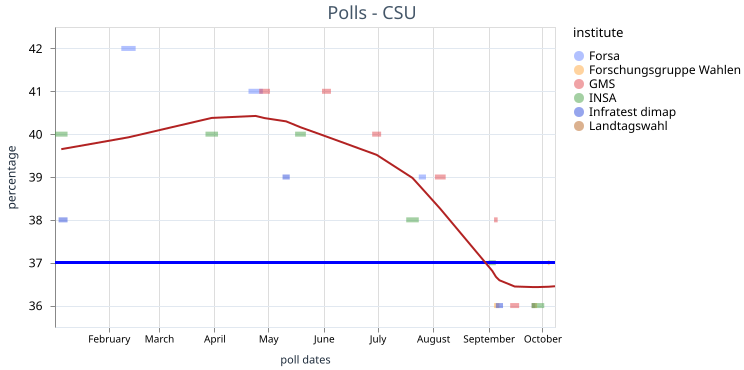
\includegraphics[width=\linewidth, keepaspectratio]{pictures/paper/polls/visualization_csu_polls.png}
\end{frame}

\begin{frame}{Polls: Freie Wähler}
	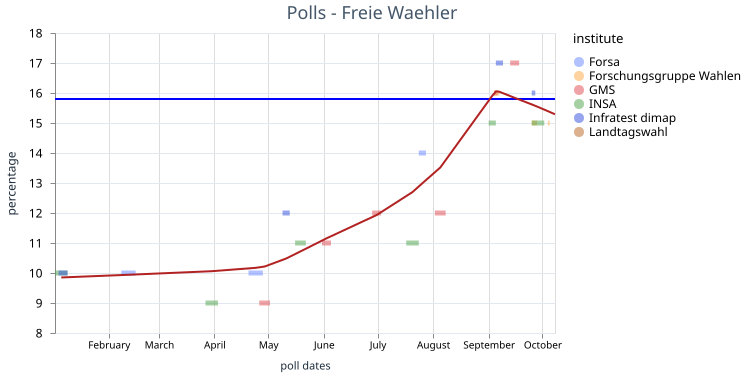
\includegraphics[width=\linewidth, keepaspectratio]{pictures/paper/polls/visualization_fw_polls.png}
\end{frame}
	
	
	\section{Lets Get some Data}
	\begin{frame}{Research Question}
		
		Predict the voting result of the 2023 Bavarian State election with Mastodon.
		
		\begin{itemize}
			\item time period: six weeks
			\item  
		\end{itemize}
		
	\end{frame}
	
	\begin{frame}{Sourcing}
		
		\begin{itemize}
			\item Search: {{instance\_url}}\/api\/v1\/timelines\/tag/{{tag\_name}}
			\begin{itemize}
				\item opt-in
				\item finished role out 2 days before election
			\end{itemize}
			\item Tags: {{isntance\_url}}\/api\/v2\/search?q={{search\_word}}
			\begin{itemize}
				\item used public timeline
			\end{itemize}
			
		\end{itemize}
	\end{frame}
	
	\begin{frame}{Data Understanding}
		
		\begin{figure}[htbp]
			\centering
			\resizebox{\columnwidth}{!}{% !TeX spellcheck = en_GB


% Define block styles
\tikzstyle{entity} = [rectangle, draw, fill=blue!20, minimum width=8em, minimum height=3em, font=\sffamily]
\tikzstyle{relationship} = [diamond, aspect=2, draw, fill=red!20, font=\sffamily]
\tikzstyle{attribute} = [ellipse, draw, fill=yellow!20, minimum width=6em, font=\sffamily]
\tikzstyle{multi attribute} = [ellipse, draw, fill=green!20, minimum width=6em, double, font=\sffamily]
\tikzstyle{line} = [draw, -latex]

\begin{tikzpicture}[auto, node distance=1.5cm]
	% Place nodes
	\node[entity] (user) {User};
	\node[attribute] (uid) [above=of user] {\underline{ID}} edge (user);
	\node[attribute] (uname) [above left=of user] {Name} edge (user);
	\node[attribute] (unote) [above right=of user] {Note} edge (user);
	\node[multi attribute] (ufields) [left=of user] {Fields} edge (user);
	
	\node[entity] (post) [right=5cm of user] {Post};
	\node[attribute] (pid) [above=of post] {\underline{ID}} edge (post);
	\node[attribute] (pdate) [below left=of post] {Date} edge (post);
	\node[attribute] (pcontent) [above right=of post] {Content} edge (post);
	
	\node[entity] (tag) [right=7cm of post] {Tag};
	\node[attribute] (tid) [above=of tag] {\underline{ID}} edge (tag);
	\node[attribute] (ttag) [above right=of tag] {Tag} edge (tag);
	
	% Place relationships
	\node[relationship] (has) [right=of user] {has} edge (user) edge (post);
	\node[relationship] (tagged) [right=of post] {tagged with} edge (post) edge (tag);
	
	% Draw edges
	\path[line] (user) -- (has);
	\path[line] (post) -- (has);
	\path[line] (post) -- (tagged);
	\path[line] (tag) -- (tagged);
\end{tikzpicture}}
			\caption{ER Diagram}
		\end{figure}
		%% !TeX spellcheck = en_GB


% Define block styles
\tikzstyle{entity} = [rectangle, draw, fill=blue!20, minimum width=8em, minimum height=3em, font=\sffamily]
\tikzstyle{relationship} = [diamond, aspect=2, draw, fill=red!20, font=\sffamily]
\tikzstyle{attribute} = [ellipse, draw, fill=yellow!20, minimum width=6em, font=\sffamily]
\tikzstyle{multi attribute} = [ellipse, draw, fill=green!20, minimum width=6em, double, font=\sffamily]
\tikzstyle{line} = [draw, -latex]

\begin{tikzpicture}[auto, node distance=1.5cm]
	% Place nodes
	\node[entity] (user) {User};
	\node[attribute] (uid) [above=of user] {\underline{ID}} edge (user);
	\node[attribute] (uname) [above left=of user] {Name} edge (user);
	\node[attribute] (unote) [above right=of user] {Note} edge (user);
	\node[multi attribute] (ufields) [left=of user] {Fields} edge (user);
	
	\node[entity] (post) [right=5cm of user] {Post};
	\node[attribute] (pid) [above=of post] {\underline{ID}} edge (post);
	\node[attribute] (pdate) [below left=of post] {Date} edge (post);
	\node[attribute] (pcontent) [above right=of post] {Content} edge (post);
	
	\node[entity] (tag) [right=7cm of post] {Tag};
	\node[attribute] (tid) [above=of tag] {\underline{ID}} edge (tag);
	\node[attribute] (ttag) [above right=of tag] {Tag} edge (tag);
	
	% Place relationships
	\node[relationship] (has) [right=of user] {has} edge (user) edge (post);
	\node[relationship] (tagged) [right=of post] {tagged with} edge (post) edge (tag);
	
	% Draw edges
	\path[line] (user) -- (has);
	\path[line] (post) -- (has);
	\path[line] (post) -- (tagged);
	\path[line] (tag) -- (tagged);
\end{tikzpicture}
		
	\end{frame}
	
	\begin{frame}{Data Understanding 2}
		\begin{figure}[htbp]
		\centering
		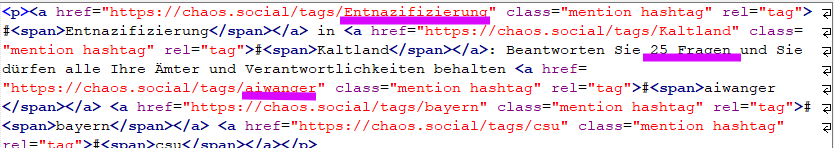
\includegraphics[width=\linewidth]{pictures/example_posts.png}
		\caption{Example Post}
		\end{figure}
	\end{frame}
	
	\begin{frame}{Data Cleaning}
		\begin{columns}
			
			\begin{column}{0.45\textwidth}
				\begin{tcolorbox}[colback=white, colframe=ElixirPurple, arc=3mm, boxrule=0mm, height=0.8\textheight, valign=center, title=Text Cleaning]
					
				\begin{itemize}
					\item html tags
					\item links
					\item special characters
					\item double spaces
				\end{itemize}
				
				
				\end{tcolorbox}
			\end{column}
			
			\begin{column}{0.45\textwidth}
				\begin{tcolorbox}[colback=white, colframe=ElixirPurple, arc=3mm, boxrule=0mm, height=0.8\textheight, valign=center, title=Post Selection]
					
					\begin{itemize}
						\item regional filter
						\begin{itemize}
							\item name local entity
							\item name any candidate
						\end{itemize}
						\item party attribution filter
												\begin{itemize}
							\item single party in post
							\item party highest frequency in post
						\end{itemize}
						\item text length
						\item double spaces
					\end{itemize}
					
					
				\end{tcolorbox}
			\end{column}
		\end{columns}
	\end{frame}
	

	
	\begin{frame}{Post Frequencies}
		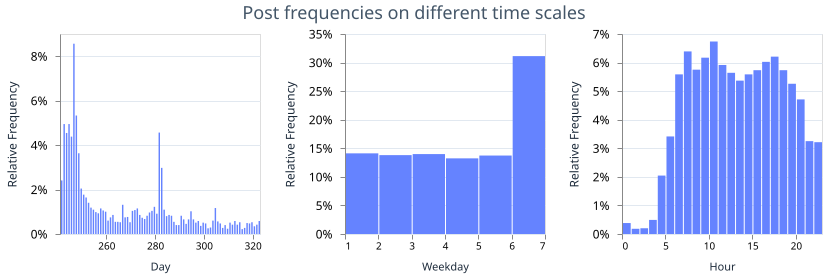
\includegraphics[width=\linewidth, keepaspectratio]{pictures/paper/sentiments/visualization_valid_posts_frequency.png}
	\end{frame}
	
	\begin{frame}{Region Classification}
		\begin{columns}
			
			\begin{column}{0.45\textwidth}
				\begin{tcolorbox}[colback=white, colframe=ElixirPurple, arc=3mm, boxrule=0mm, height=0.8\textheight, valign=center, title=Text Cleaning]
					\begin{figure}[htbp]
						\centering
						\resizebox{\columnwidth}{!}{% !TeX spellcheck = en_GB

% Define block styles
\tikzset{
	decision/.style={
		diamond, 
		draw, 
		fill=blue!20, 
		text width=4.5em, 
		text badly centered, 
		node distance=2cm, 
		inner sep=0pt
	},
	block/.style={
		rectangle, 
		draw, 
		fill=blue!20, 
		text width=5em, 
		text centered, 
		rounded corners, 
		minimum height=4em
	},
	line/.style={
		draw, 
		-{Latex[length=3mm,width=3mm]}, 
		thick
	},
	decisionarrow/.style={
		draw, 
		-{Latex[length=3mm,width=3mm]}, 
		thick, 
		decorate, 
		decoration={snake, amplitude=.2mm, segment length=2mm, post length=1mm}
	}
}

\begin{tikzpicture}[node distance=2.5cm and 2.5cm, auto, every node/.style={font=\Large}]
	% Place nodes
	\node [decision] (bavinstance) {Bavarian Instance?};
	\node [decision,below right=1cm of bavinstance] (bavfield) {Bavarian Location in Field?};
	\node [decision, below right=1cm of bavfield] (bavusernote) {Bavarian Location in User note?};
	\node [decision, below right=1cm of bavusernote] (inferlang) {Language is German?};
	\node [block, left=3.5cm of inferlang, node distance=2.5cm] (german) {German};
	\node [block, right=1.5cm of inferlang, node distance=3cm] (foreign) {Foreign};
	\node [block, left of=german, node distance=4cm] (bavarian) {Bavarian};
	
	% Draw edges
	\draw [line] (bavinstance) -- node [near start] {no} (bavfield);
	\draw [line] (bavfield) -- node [near start] {no} (bavusernote);
	\draw [line] (bavusernote) -- node [near start] {no} (inferlang);
	\draw [line] (inferlang) -- node [near start] {yes} (german);
	\draw [line] (inferlang) -- node [near start] {no} (foreign);
	\draw [decisionarrow] (bavfield.west) -| node [near start, above] {yes} (bavarian);
	\draw [decisionarrow] (bavusernote.west) -| node [near start, above] {yes} (bavarian);
	\draw [decisionarrow] (bavinstance.west) -| node [near start, above] {yes} (bavarian);
\end{tikzpicture}
}
						\caption{High Level}
					\end{figure}
				%% !TeX spellcheck = en_GB

% Define block styles
\tikzset{
	decision/.style={
		diamond, 
		draw, 
		fill=blue!20, 
		text width=4.5em, 
		text badly centered, 
		node distance=2cm, 
		inner sep=0pt
	},
	block/.style={
		rectangle, 
		draw, 
		fill=blue!20, 
		text width=5em, 
		text centered, 
		rounded corners, 
		minimum height=4em
	},
	line/.style={
		draw, 
		-{Latex[length=3mm,width=3mm]}, 
		thick
	},
	decisionarrow/.style={
		draw, 
		-{Latex[length=3mm,width=3mm]}, 
		thick, 
		decorate, 
		decoration={snake, amplitude=.2mm, segment length=2mm, post length=1mm}
	}
}

\begin{tikzpicture}[node distance=2.5cm and 2.5cm, auto, every node/.style={font=\Large}]
	% Place nodes
	\node [decision] (bavinstance) {Bavarian Instance?};
	\node [decision,below right=1cm of bavinstance] (bavfield) {Bavarian Location in Field?};
	\node [decision, below right=1cm of bavfield] (bavusernote) {Bavarian Location in User note?};
	\node [decision, below right=1cm of bavusernote] (inferlang) {Language is German?};
	\node [block, left=3.5cm of inferlang, node distance=2.5cm] (german) {German};
	\node [block, right=1.5cm of inferlang, node distance=3cm] (foreign) {Foreign};
	\node [block, left of=german, node distance=4cm] (bavarian) {Bavarian};
	
	% Draw edges
	\draw [line] (bavinstance) -- node [near start] {no} (bavfield);
	\draw [line] (bavfield) -- node [near start] {no} (bavusernote);
	\draw [line] (bavusernote) -- node [near start] {no} (inferlang);
	\draw [line] (inferlang) -- node [near start] {yes} (german);
	\draw [line] (inferlang) -- node [near start] {no} (foreign);
	\draw [decisionarrow] (bavfield.west) -| node [near start, above] {yes} (bavarian);
	\draw [decisionarrow] (bavusernote.west) -| node [near start, above] {yes} (bavarian);
	\draw [decisionarrow] (bavinstance.west) -| node [near start, above] {yes} (bavarian);
\end{tikzpicture}

				\end{tcolorbox}
			\end{column}
			
			\begin{column}{0.45\textwidth}
				\begin{tcolorbox}[colback=white, colframe=ElixirPurple, arc=3mm, boxrule=0mm, height=0.8\textheight, valign=center, title=Post Selection]
					
					\begin{figure}[htbp]
						\centering
						\resizebox{\columnwidth}{!}{% !TeX spellcheck = en_GB

% Define block styles
\tikzstyle{block} = [rectangle, draw, fill=blue!20, text width=15em, text centered, rounded corners, minimum height=3em, drop shadow]
\tikzstyle{line} = [draw, -latex, line width=0.7mm,]

\begin{tikzpicture}[node distance=3.0cm and 2cm, auto, every node/.style={font=\Huge}] % Adjusted node distance for wider separation
	% Nodes
	\node [block] (init) {XLM-RoBERTa};
	%\node [block, below left=2cm and 3cm of init] (german) {German}; % Position adjusted for wider layout
	%\node [block, below right=2cm and 3cm of init] (english) {English}; % Position adjusted for wider layout
	\node [block, below left=3cm and 3cm of init] (germanbert) {german-sentiment\_bert};
	\node [block, below right=3cm and 3cm of init] (roberta) {RoBERTa BERTweet - Sentiment};
	\node [block, below=3cm of germanbert] (bavarianq1) {Bavarian?};
	\node [block, below=3cm of roberta] (bavarianq2) {Bavarian?};
	\node [block, below=3cm of bavarianq1] (german2) {German}; % Position adjusted for separation
	\node [block, below=3cm of bavarianq2] (english2) {English}; % Position adjusted for separation
	\node [block, below right=3cm and 1cm of bavarianq1] (bavarian) {Bavarian}; % Position adjusted for separation
	
	% Edges
	\path [line] (init) -| node [near start] {German} (germanbert);
	\path [line] (init) -| node [near start] {English} (roberta);
	%\path [line] (german) -- (germanbert);
	%\path [line] (english) -- (roberta);
	\path [line] (germanbert) -- (bavarianq1);
	\path [line] (roberta) -- (bavarianq2);
	\path [line] (bavarianq1) -- node [near start, right] {yes} (bavarian);
	\path [line] (bavarianq1) -- node [near start, left] {no} (german2);
	\path [line] (bavarianq2) -- node [near start, left] {yes} (bavarian);
	\path [line] (bavarianq2) -- node [near start, right] {no} (english2);
\end{tikzpicture}
}
						\caption{High Level}
					\end{figure}
					%% !TeX spellcheck = en_GB

% Define block styles
\tikzstyle{block} = [rectangle, draw, fill=blue!20, text width=15em, text centered, rounded corners, minimum height=3em, drop shadow]
\tikzstyle{line} = [draw, -latex, line width=0.7mm,]

\begin{tikzpicture}[node distance=3.0cm and 2cm, auto, every node/.style={font=\Huge}] % Adjusted node distance for wider separation
	% Nodes
	\node [block] (init) {XLM-RoBERTa};
	%\node [block, below left=2cm and 3cm of init] (german) {German}; % Position adjusted for wider layout
	%\node [block, below right=2cm and 3cm of init] (english) {English}; % Position adjusted for wider layout
	\node [block, below left=3cm and 3cm of init] (germanbert) {german-sentiment\_bert};
	\node [block, below right=3cm and 3cm of init] (roberta) {RoBERTa BERTweet - Sentiment};
	\node [block, below=3cm of germanbert] (bavarianq1) {Bavarian?};
	\node [block, below=3cm of roberta] (bavarianq2) {Bavarian?};
	\node [block, below=3cm of bavarianq1] (german2) {German}; % Position adjusted for separation
	\node [block, below=3cm of bavarianq2] (english2) {English}; % Position adjusted for separation
	\node [block, below right=3cm and 1cm of bavarianq1] (bavarian) {Bavarian}; % Position adjusted for separation
	
	% Edges
	\path [line] (init) -| node [near start] {German} (germanbert);
	\path [line] (init) -| node [near start] {English} (roberta);
	%\path [line] (german) -- (germanbert);
	%\path [line] (english) -- (roberta);
	\path [line] (germanbert) -- (bavarianq1);
	\path [line] (roberta) -- (bavarianq2);
	\path [line] (bavarianq1) -- node [near start, right] {yes} (bavarian);
	\path [line] (bavarianq1) -- node [near start, left] {no} (german2);
	\path [line] (bavarianq2) -- node [near start, left] {yes} (bavarian);
	\path [line] (bavarianq2) -- node [near start, right] {no} (english2);
\end{tikzpicture}

				\end{tcolorbox}
			\end{column}
		\end{columns}
	\end{frame}
	
	
\begin{frame}{Sentiment analysis}
	todo: show example
\end{frame}
	
\end{document}

